\documentclass[twocolumn, 10pt]{article}
\usepackage[left=2.5cm,right=2.5cm,top=3.0cm,bottom=3cm,a4paper]{geometry}
\setlength{\columnsep}{1cm}
\usepackage[utf8]{inputenc}
\usepackage{times}
\usepackage{CJKutf8}
\usepackage{amsmath}
\usepackage{float}
\usepackage{multirow,makecell}
\usepackage{tabularx}
\usepackage{lipsum}                  % http://ctan.org/pkg/lipsum
\usepackage{latexsym}
\usepackage{url}
\usepackage{times}
\usepackage{multirow,makecell}
\usepackage{hyperref}                % NOTE(lucypark): for \autoref
\usepackage{subcaption}              % NOTE(lucypark): for subfigures 
\usepackage{graphicx}                % http://ctan.org/pkg/graphicx
\DeclareGraphicsExtensions{.pdf,.png,.jpg}
\usepackage{enumitem} 
\pagenumbering{gobble}


% 밑의 주석의 코드들은 section, subsection 을 양식에 맞추기 위한 코드입니다. default 값이 아닌 예를 들어 Bold체의 section font를 사용해야 한다거나 이럴 경우 사용하는 패키지입니다.
% \usepackage{titlesec}
% \titleformat*{\section}{\bfseries}
% \titleformat*{\subsection}{\bfseries}
% \titleformat*{\subsubsection}{\bfseries}
% \titleformat*{\paragraph}{\bfseries}
% \titleformat*{\subparagraph}{\bfseries}


\usepackage[square,numbers]{natbib}
\bibliographystyle{unsrtnat}
\begin{document}
\begin{CJK}{UTF8}{}
\CJKfamily{mj}
\title{How to make latex paper?}
\author{Name \\
        TEAMLAB \\
        teamlab.gachon@gmail.com\\}

% \data{} 는 제목 저자의 정보 밑에 기술한 날짜가 default 값으로 showing 됩니다. data를 기술하지 말하야 하는 경우라면 밑의 코드를 적어주세요.
\date{}  

% 논문의 제목 저자의 정보를 나타냅니다.
\maketitle   

% 논문의 Section 을 시작합니다. 
\begin{abstract}
논문의 Abstract 입니다. 
\end{abstract}


\section{Introduction}
논문의 도입부를 적습니다. 

\section{How to make subsection}
\subsection{subsection}
sub section을 사용하는 방식은 section 시작 하단 부에 다음과 같이 적으면 됩니다.
\begin{verbatim}
 \subsection{적고자 하는 내용}    
\end{verbatim}


\section{How to get citation}
논문을 작성할 때 인용을 해야하는 상황이 많이 있습니다. 인용정보를 latex 에서는 아주 쉽게 이용할 수 있습니다. 
우선 Google의 학술검색 https://scholar.google.co.kr/ 에 접속하여 원하는 논문을 검색합니다. 

\begin{figure}[h]
    \centering
    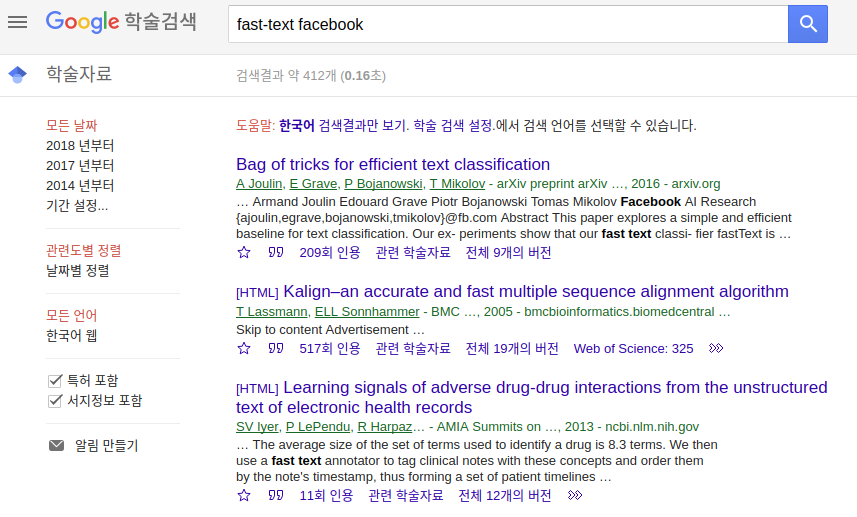
\includegraphics[scale=0.23]{figure/fast-text.png}
    \caption{학술검색 결과}
    \label{fig:figure1}
\end{figure}

예를 들어 fast-text를 검색할 경우 \autoref{fig:figure1} 과 같은 화면을 볼 수 있습니다. 그 후 해당하는 논문에서 큰 따옴표 표시가 된 곳을 클릭합니다.

\begin{figure}[h]
    \centering
    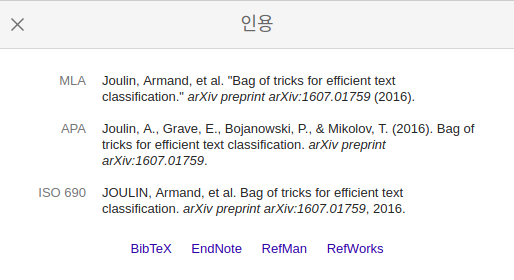
\includegraphics[scale=0.35]{figure/fast-text2.png}
    \caption{인용아이콘 클릭시}
    \label{fig:figure2}
\end{figure}

\autoref{fig:figure2} 화면이 보이게 되면 우리가 사용하는 툴이 latex기 때문에 가장 왼쪽의 BibTeX를 클릭합니다.

\begin{figure}[h]
    \centering
    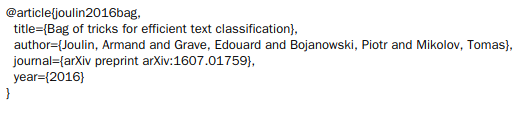
\includegraphics[scale=0.35]{figure/fast-text3.png}
    \caption{인용정보}
    \label{fig:figure3}
\end{figure}

\autoref{fig:figure3} 의 인용정보를 복사합니다. 그 후 latex로 돌아와서 xxxx.bib 이라는 인용정보를 담아두는 공간에 붙여넣기를 해줍니다. 
그 후 원하는 글옆에 다음과 같은 코드를 넣어줍니다. 
\begin{verbatim}
 \cite{Einstein}.   
\end{verbatim}
인용을 여기에 붙이게 되면\cite{Einstein} 이 됩니다.

\section{Mathematical representation}
수식을 적는 방법은 다음과 같습니다. 
\begin{equation}
a = W \times X
\end{equation}
이 방식 외에서 글 옆에 표시해야 하는 경우가 종종 있는데 그럴경우 $a = W \times X$ 와 같이 적어줍니다.
\begin{verbatim}
  % 수식을 중앙에 표시
  \begin{equation} 
    a = W \times X
  \end{equation}  
  % inline 수식
  $ a = W \times X $
\end{verbatim}

\section{Table}
논문에서 Table은 빈번하게 사용됩니다.

\begin{table}[ht]
\begin{center}
\resizebox{\columnwidth}{!}{%
   \begin{tabular}{|l|r|r|r|r|r|r|r|r|}
   \hline
    & A & B & C & D & E & F & G & H \\ \hline
   N & 1 & 2 & 3 & 4 & 5 & 6 & 7 & 8 \\\hline
   \end{tabular}%
   }
   \end{center}
\caption{\label{tab:table1} 이곳에 Table의 설명을 적으세요.}
\end{table}
코드를 살펴보면, 

\begin{verbatim}
\begin{table}[h]
\begin{center}
\resizebox{\columnwidth}{!}{%
   \begin{tabular}{|l|r|r|r|r|r|}
   \hline
    & A & B & C & D & E \\ \hline
   N & 1 & 2 & 3 & 4 & 5 \\\hline
   \end{tabular}%
   }
   \end{center}
\caption{\label{tab:table1} write..}
\end{table}
\end{verbatim}

\autoref{tab:table1} 의 코드를 보면 첫번 째줄에서 table을 시작하고 [h]는 현재 table이 들어가기에 공간이 충분하다면 그 곳에 table을 지정하겠다는 뜻입니다. 
대문자 H의 경우 강제지정입니다. 3번째 코드는 columns 개수만큼 width의 공간을 fit 하겠다는 것이고 $|\, l\,|r|\cdots|r| $ 은 table 안의 text-align을 정하는것입니다.
$l$은 left $c$ 는 center $r$ 은 right 입니다. column은 $&$로 구분되어 집니다. 


\section{Figure}
이미지를 지정하는 방식은 다음과 같습니다. 
\begin{verbatim}
\begin{figure}[h]
    \centering
    \includegraphics[scale=0.23] \\
    {figure/fast-text.png}
    \caption{write..}
    \label{fig:figure1}
\end{figure}
\end{verbatim}

scale의 부분은 이미지의 크기를 나타내며 다음 대괄호는 path입니다. label 은 우리가 이 이미지를 설명할 때 reference를 사용해서 \autoref{fig:figure1} 와 같이 나타냅니다.

\section{Grammar}
latex에서 자주 사용하는 문법은 다음과 같습니다.

\begin{enumerate}[label=(\roman*)]
  \item First item
  \item Second item
  \item Third item
\end{enumerate}
\begin{verbatim}
  \begin{enumerate}[label=(\roman*)]
    \item First item
    \item Second item
    \item Third item
  \end{enumerate}
\end{verbatim}


\underline{underline}
\begin{verbatim}
    \underline{underline}
\end{verbatim}

$i \in (1, 30)$
\begin{verbatim}
    $i \in (1, 30)$
\end{verbatim}

$ A \times B$
\begin{verbatim}
    $A \times B$
\end{verbatim}

$ A \cdots B$
\begin{verbatim}
    $ A \cdots B$
\end{verbatim}

$ \frac{A}{B}$
\begin{verbatim}
    $ \frac{A}{B} $
\end{verbatim}

$ e^{x}$
\begin{verbatim}
    $ e^{x}$
\end{verbatim}

$ e_{1}$
\begin{verbatim}
    $ e_{1} $
\end{verbatim}

\section{Acknowledge}
논문의 사사를 적는곳입니다.


\end{CJK}

\medskip

\bibliography{sample}

\end{document}







